\documentclass[11pt]{article}
\usepackage{amsmath}
\usepackage[sc]{mathpazo} %Like Palatino with extensive math support
\usepackage{fullpage}
%\usepackage[authoryear,sectionbib,sort]{natbib}
\usepackage[square,sort,comma,numbers]{natbib}
\linespread{1.7}
\usepackage[utf8]{inputenc}
\usepackage{lineno}
\usepackage{titlesec}
\usepackage{xcolor}
\usepackage{graphicx}
\usepackage{placeins}
\usepackage{float}
\usepackage{subfigure}
\newcommand{\tom}[2]{{\color{red}{#1}}\footnote{\textit{\color{red}{#2}}}} 
\newcommand{\ali}[2]{{\color{blue}{#1}}\footnote{\textit{\color{blue}{#2}}}}  


\titleformat{\section}[block]{\Large\bfseries\filcenter}{\thesection}{1em}{}
\titleformat{\subsection}[block]{\Large\itshape\filcenter}{\thesubsection}{1em}{}
\titleformat{\subsubsection}[block]{\large\itshape}{\thesubsubsection}{1em}{}
\titleformat{\paragraph}[runin]{\itshape}{\theparagraph}{1em}{}[.]\renewcommand{\refname}{Literature Cited}


%%%%%%%%%%%%%%%%%%%%%
% Line numbering
%%%%%%%%%%%%%%%%%%%%%
%
% Please use line numbering with your initial submission and
% subsequent revisions. After acceptance, please turn line numbering
% off by adding percent signs to the lines %\usepackage{lineno} and
% to %\linenumbers{} and %\modulolinenumbers[3] below.
%
% To avoid line numbering being thrown off around math environments,
% the math environments have to be wrapped using
% \begin{linenomath*} and \end{linenomath*}
%
% (Thanks to Vlastimil Krivan for pointing this out to us!)

\title{Thank you, next: demographic consequences of partner diversity and turnover in a multi-species ant-plant mutualism}
% title suggestion, trying to move away from focus on IPM

\author{Alexandra Campbell$^{1,\dagger}$ \\ 
	Tom E.X. Miller$^{1,\ast}$}

\date{}

\begin{document}
	
	\maketitle
	
	\noindent{} 1. Program in Ecology and Evolutionary Biology, Department of BioSciences, Rice University, Houston, Texas 77005;
	
	\noindent{} $\dagger$ e-mail: amc49@rice.edu\\
	\noindent{} $\ast$ e-mail: tom.miller@rice.edu
	
	\bigskip
	
	\textit{Keywords}:  Integral Projection Model, \textit{Cylindropuntia imbricata}, population fitness, multi-species mutualism, complementarity, sampling effect, portfolio effect
	
	\bigskip
	
	\textit{Manuscript type}: Article.
	
	\bigskip
	
	\noindent{\footnotesize Prepared using the suggested \LaTeX{} template for \textit{Am.\ Nat.}}
	
\linenumbers{}
\modulolinenumbers[3]

\newpage{}

	\section*{Abstract}
% 200 words max
The diversity of partners in a multi-species mutualism causes varied demographic effects on the population of the focal mutualist which can be explained by several mechanisms: portfolio effect, complementarity, and sampling effect.
\textit{Cylindropuntia imbracata} (tree cholla) produce extrafloral nectar and various ant partners provide defense from herbivores and seed predators. 
We used plant demographic censuses to parameterize a series of Bayesian hierarchical generalized linear vital rate models to determine the impacts of different partners on the focal mutualists. 
We constructed an Integral Projection Model in which we simulate different combinations of ant partners that don’t occur in the wild.
The hierarchical models revealed that different ant partners had different impacts on the cholla vital rates. 
Specifically, \textit{C. opuntiae} tended plants had advantages in both growth and survival when small, and large \textit{L. apiculatum} tended plants had floral viability advantages. 
The IPM results revealed that scenario which included \textit{L. apiculatum} only resulted in the highest possible fitness for the tree cholla. 
This suggests that there are no benefits of diversity in this system.
This study highlights that partner diversity does not always increase the benefits a focal mutualist receives.

\newpage{}
\section*{Introduction}
Mutualisms are species interactions where all participants receive net benefits, leading to higher individual fitness and increased population growth rates. 
\tom{They are widespread species interactions \citep{Bronstein1994,Chamberlain2014,Frederickson2013,Axelrod1981,Leigh2010} but can deteriorate into commensalism or parasitism under conditions that elevate costs or dampen benefits \citep{Rodriguez-Rodriguez2017,Song2020,Mandyam2014,Thrall2007, Bahia2022}.}{I suggest condensing the two sets of citations into one at the end of the sentence. The states that they are widespread species interactions is so broad and vague that it is not really worth citing.}
Mutualisms are considered more context dependent than other species interactions \citep{Chamberlain2014,Frederickson2013}, meaning the magnitude and sign of interaction strength are often determined by environmental conditions and species' identities \citep{Noe1994,Leigh2010}.

Mutualism is defined at the level of a species pair (+/+) but these interactions are embedded within multi-species communities, and growing evidence suggests that pairwise interactions are poor predictors of the net effects of multi-species mutualism \citep{Afkhami2014,Palmer2010,Bascompte2009,Dattilo2014}. 
A focal mutualist may interact with multiple guilds of partner types (e.g., plants that interact with pollinators, seed dispersers, soil microbes, and ant defenders) or with multiple partner species within the same guild (e.g., plants visited by multiple pollinator species). 
Within a mutualist guild, partner species often differ in the amount or type of goods or services they provide, making partner identity an important source of contingency in mutualism \citep{Stanton2003}. 
Whether and how partner diversity modifies the demographic effects of mutualistic interactions remain open questions within relevance in applied settings \citep{rogers2014, Thibaut2012, Frederickson2005, Palmer2010}.

There are multiple mechanisms by which partner diversity can influence the net benefits accrued by a focal mutualist, mirroring the mechanisms by which, at a larger scale of organization, biodiversity can influence ecosystem function \cite{Yeung2006,Barrett2015,Ushio2020}. 
First, when there is a hierarchy of fitness effects (a consistent ranking of best to worst mutualists), a more diverse sample of the partner community may be more likely to include the best partner \cite{Frederickson2013}.
This can lead to an apparent benefit of diversity driven by a sampling effect \cite{Batstone2018} -- but there is no benefit of diversity \emph{per se}, only better and worse partners. 
If partner associations are mutually exclusive (a focal mutualist may engage with only one partner at a time), then partner diversity may impose opportunity costs, leading to negative effects of a diverse mutualist assemblage relative to exclusive association with the single best partner \citep{Miller2007}. 
Second, even within a single mutualist guild, the benefits conferred by alternative partner species can vary in type and not just degree \cite{Stachowicz2005,Bronstein2006,Stanton2003}. 
This can lead to a positive effect of partner diversity through complementarity of alternative functions \cite{Batstone2018}. 
Interference or synergies between partners can make their combined effect different than the expected from the sum of complementary functions \cite{Afkhami2014}. 
Third, partner species can have species-specific responses to environmental variation, either spatially \citep{Ollerton2006} or temporally \citep{Alarcon2008}. 
Multiple partners can therefore act as a 'portfolio' that stabilizes fitness benefits across spatial or temporal heterogeneity, leading to positive effects of partner diversity through the portfolio effect \cite{Batstone2018,Lazaro2022,Horvitz1990}. 

Partner diversity can have different effects depending on whether partners are present simultaneously or sequentially (partner turnover) \citep{Djieto-Lordon2005, Ness2006, Bruna2014,Barrett2015,Ushio2020,Dattilo2014}. 
Sequential associations are likely when alternative partners engage in interference competition for access to a shared mutualist \cite{Kiers2003,Batstone2018,Tgaard2015,Wulff2008}. 
Turnover can happen at different timescales, from minutes to years \citep{Oliveira1999,Horvitz1986}. 
The frequency of partner turnover can impact the level of benefits received by the focal mutualist, particularly if the benefits continue to accumulate with successive turnover (e.g., when sequential partners provide complementary functions) or if they saturate over time \citep{Sachs2004,Fiala1994}.
Directionality of turnover can also influence effects of partner diversity if partner identity changes consistently across ontogeny of a focal mutualist \citep{Fonseca2003,Noe1994,Dejean2008}.
For example, plant susceptibility to enemies can change across life stages \citep{Boege2005,Barton2010}, so the benefits of a diverse guild of defensive mutualists are greatest when more defensive partner species align with more vulnerable life stages \citep{Djieto-Lordon2005,Dejean2008}.

Defensive ant-plant mutualisms -- where plants provide food and/or housing to ants that in turn defend them from enemies -- are widespread interactions that offer valuable model systems for the ecology and evolution of mutualism \citep{Bronstein1998, Bronstein2006}. 
Extrafloral nectar (EFN) -bearing plants can serve as dietary resources that promote ant abundance and colony size \citep{Byk2011, Ness2009, Ness2006, Donald2022}.
In turn, presence of defensive ant partners is often linked to reductions in herbivory  \citep{Trager2010, Rudgers2004} and demographic advantages for the plant partner \citep{Baez2016}.
Defensive ant-plant mutualisms are commonly multi-species, where a guild of ant partner species share, and often compete for, a plant mutualist \citep{Bronstein1998, Beattie1985, Trager2010, Agrawal1998}.
Ant partners can vary in their ability to deter herbivores \citep{Bruna2014}, and visitation by low quality ant partners can prevent visitation by higher quality partners, consequently causing a reduction in fitness through missed opportunity costs \citep{Fraser2001, Frederickson2005}.
Susceptibility to herbivory can also vary significantly throughout the life stages of the plant \citep{Boege2005}, suggesting that the order and timing of successive partners is important to the fitness impacts of the combined partner guild \citep{Barton2010, Boege2005, Fonseca2003}.
Finally, herbivore identity and pressure can vary inter-annually \cite{Wetzel2023}, much like mutualist identity and presence, meaning the threat plants face can vary just as much as the protection they receive due to temporal stochasticity. 
Previous studies have investigated how ant partner diversity affects plant fitness \citep{Palmer2010,Afkhami2014,Fiala1994,Gaume1998,Dattilo2014,Ludka2015}
However, little is known about the combined effects of partner identity, directional partner turnover, and temporal stochasticity, particularly because the necessary long-term data are rarely available. 
	
This study examined the consequences of partner diversity in a food-for-protection mutualism between the tree cholla cactus (\textit{Cylindriopuntia imbricata}), a long-lived EFN-bearing plant, and multiple species of ant partners.
Previous studies have shown that herbivory by specialized insect herbivores negatively affects cactus fitness \cite{Miller2009}, and that ant defense reduces herbivore damage \cite{Miller2007}. 
Tree cholla are tended by two common ant species (\textit{Liometopum apiculatum} and \textit{Crematogaster opuntiae}) and several additional rarer species, all of which collect EFN during foraging visits but their colonies are ground-nesting and not housed by the plants. 
These ant species locally co-occur but individual plants are typically tended by only one species that patrols the plant around-the-clock and maintains control of the plant's nectar resources, usually for an entire growing season \citep{Ohm2014, Donald2022}. 
Switches between partner species, or between vacancy and ant occupancy, commonly occur from one growing season to the next \citep{Miller2007}. 
Prior experiments suggested a hierarchy of mutualist quality, with \textit{L. apiculatum} providing strong anti-herbivore defense and \textit{C. opuntiae} having net negative effects because herbivore deterrence is outweighed by deterrence of pollinators \citep{Miller2007,Ohm2014}. 
However, all of our previous studies in this system have focused on single life stages (adult plants) or vital rates (seed production) and did not integrate the demographic effects of ant defense across the life cycle, which may be essential for understanding net fitness effects of a diverse partner guild \citep[e.g.,][]{Palmer2010}. 
To our knowledge no previous study has incorporated inter-annual stochasticity into models of ant-plant dynamics, which limits our understanding of diversity benefits that may arise through the portfolio effect. 

Here we used a unique long-term data set that allows us to explore mutualistic associations with multiple partner species, longitudinal turnover in partner identity, and how the demographic effects of alternative partners varies across plant size structure and nearly 20 years of inter-annual fluctuations. 
We used this observational data set of plant demography and ant-plant associations, contextualized by previous ant exclusion experiments, to investigate whether and through which mechanism(s) partner diversity affects the fitness benefits of ant visitation. 
Specifically, we asked:
	\begin{enumerate}	
		\item{What are the demographic effects of association with alternative partners and how do these effects fluctuate across years?}
		\item{What are the frequency and direction of partner turnover across the plant life cycle?}	
		\item{What is the net effect of partner diversity on plant fitness, and what mechanism(s) explain(s) this effect?}
	\end{enumerate}
To answer these questions we used a hierarchical Bayesian statistical approach to estimate demographic vital rates for hosts in different states of ant occupancy and to quantify state-dependent partner turnover from the long-term data. 
We then used a stochastic, multi-state integral projection model (IPM) that combines diverse effects on vital rates and pathways of partner turnover to quantify effects of partner diversity on plant fitness. 


\section*{Methods}
\subsection*{Study System}
  
This study was conducted in the Los Pi$\tilde{n}$os mountains, a small mountain chain located on the Sevilleta National Wildlife Refuge, a Long-term Ecological Research site (SEV-LTER) in central New Mexico, USA.
This is an area characterized by steep, rocky slopes, and perennial vegetation including grasses (\textit{Bouteloua eriopoda} and \textit{B. gracilis}), yuccas, cacti, and junipers. 
Tree cholla cacti are common in high Chihuahuan desert habitats, with their native range spanning the southwestern USA \citep{Benson1982}. 
These arborescent plants produce cylindrical segments with large spines. 
In the growing season (May to August in New Mexico), the plants initiate new vegetative segments and flower buds at the ends of existing segments. 
While most plants produce new segments every season, only those which are reproductively mature produce flower buds. 
%Tree cholla generally reach at least 9 years of age before beginning to reproduce \citep{Ohm2014}.
Like other EFN-bearing cacti, tree cholla secrete nectar from specialized glands on young vegetative segments and flower buds \citep{Ness2006,Oliveira1999}. 
Flower buds produce more and higher-quality EFN than vegetative segments, making reproductive cholla valuable mutualist partners \citep{Miller2014}. 
%Smaller cholla produce little to no EFN, so larger cholla, especially flowering individuals, are generally more highly tended. 

Tree cholla EFN is harvested by various ant species. 
At SEV-LTER, cholla are visited primarily by two species of ground-nesting ants, \textit{Crematogaster opuntiae} and \textit{Liometopum apiculatum}, as well as other rarer species, including \textit{Forelius pruinosus} and unidentified species in the genera \textit{Aphaenogaster} and \textit{Camponotus}.
\textit{L. apiculatum} are the most frequent visitors with $25\% - 60\%$ of tree cholla tended by these ants, followed by \textit{C. opuntiae} visiting between $5\% - 20\%$ of cacti depending on the year \citep{Donald2022}. 
Between $ 30\% - 80\%$ of cacti remain vacant in any given year. 
Workers of different species rarely co-occur on individual plants, likely due to interspecific competition \citep{Miller2007}: staged introductions of \textit{C. opuntiae} to \textit{L. apiculatum}-tended plants, and vice versa, provoke aggressive responses by residents (A. Cambpell, \textit{personal observation}).
%Each cholla is visited by a single ant species for the duration of a season, and the species of the visitors can change from one season to the next. 
In Fall, tree cholla stop producing EFN and the ants vacate until the next growing season. 

Multiple insect herbivores and seed predators specialize on tree cholla \citep{Mann1969}. 
The Cerambycid beetle \textit{Moneilema appressum} and a weevil (Coleoptera: Curculionidae) of the genus \textit{Gerstaekeria} feed on vegetative and reproductive structures as adults and their larvae feed internally. 
A cactus bug, \textit{Narnia pallidicornis} (Hemiptera: Coreidae), feeds on all cholla parts with a preference for the reproductive structures \citep{Miller2006}.
A seed predator, \textit{Cahela ponderosella} (Lepidoptera: Pyralidae), oviposits in open flowers and larvae eat seeds in developing fruits. 
These predators can have significant negative impacts on plant fitness of and depress population growth \citep{Miller2009}.
Prior experiments showed that ant-tended tree cholla experience less herbivory and seed predation than plants from which ants were excluded \citep{Miller2007,Ohm2014}. 

\subsection*{Data Collection}
This study is based on long-term demographic data spanning 2004 to 2023 at SEV-LTER. 
From 2004 to 2008, we censused 134 plants distributed across three spatial blocks. 
This initial census group was discontinued in 2009, when we established six 30 $\times$ 30-meter plots and tagged all tree cholla within those plots. 
Two additional 30 $\times$ 30-meter plots were added in 2011, and this group of eight plots has since been censused annually through 2023 (with the exception of 2020 due to the pandemic shutdown). 
For all plants, in May or early June of each year we recorded plant survival since the last survey and, for survivors, we recorded height (cm), maximum crown width (cm), and crown width perpendicular to the maximum (cm).
Size measurements were used to calculate plant volume ($cm^3$) based on the volume of an elliptical cone. 
We measured reproduction as counts of viable and aborted flowerbuds. 
We recorded the ant species present (or vacancy if no ants present).
Occurrences of more than one ant species on one plant were rare (less than 5\% of observations), and for the purpose of this analysis we classified the plant as being occupied by the more abundant species. 
Plots were searched for new recruits each year, and these were added to the census.
In total, the data set included 1141 unique individuals and 19 year observations. 
%These data were used to fit vital rate models (survival, growth, reproduction) as functions of plant size and ant occupancy state. 

We used additional, smaller data sets from previously published studies to estimate seed and seed bank parameters. 
Ohm et al. \citeyear{Ohm2014} provide data on the number of seeds per fruit for plants tended by \textit{L. apiculatum}, \textit{C. opuntiae}, or no ants (experimental exclusion), accounting for their effects on pollinator visitation. 
Elderd and Miller \citeyear{elderd2016quantifying} provide data on seed entry to the seed bank and seedling germination and survival rates. 


\subsection*{Multi-state Integral Projection Model}
Integral Projection Models describe population dynamics in discrete time, with functions that relate vital rates to continuous state variables \citep{ellnerbook}. 
While IPMs are a natural choice for populations with continuous size structure, they can also be modified to accommodate a combination of continuous and discrete state variables, as we do here. 
We constructed a stochastic, multi-state IPM that stitches together population structure associated with plant size and ant state, allowing us to determine the individual fitness effects of each ant species and the composite effects of multiple partners, with ant transition dynamics and inter-annual variability modeled explictly. 

Given the low frequency of ant occupancy states other than \textit{L. apiculatum} and \textit{C. opuntiae} (\textless8\% of observations) we combined all other ants into an ``other'' category, such that our multi-state IPM included four ant states: vacant, \textit{L. apiculatum}, \textit{C. opuntiae}, and Other. 
The ``Other'' category was made up of \textit{Forelius pruinosus} (3.5\% of observations), unidentified species belonging to the genera \textit{Camponotus} (0.9\%), \textit{Aphaenogaster} (0.4\%), \textit{Myrmecocystus} (0.08\%), \textit{Tetramorium} (0.02\%), \textit{Brachymyrmex} (0.02\%), and additional ants not identified to genus or species (2.8\%). 

Ant state is included as a predictor variable in IPM sub-models where there are biologically realistic pathways through which ants could impact the outcome of that process. 
For example, ant partners defend cacti from herbivores, and prior experimental work indicates that ant tending can reduce vegetative tissue loss and floral abortion.
Therefore, ant state was included in sub-models for survival, growth, and flowerbud viability. 
In contrast, we have no reason to expect that ant tending can directly influence the probability of flowering or flowerbud production independently of its influence on plant size, so these sub-models do not include ant state as a predictor variable. 

We modeled the tree cholla life cycle using continuously size-structured plants where $n(x,a)_{t}$ gives the number of plants of size $x$  and ant state $a$ in year $t$, plus two discrete seed banks ($B^1_{t}$ and $B^2_{t}$) corresponding to 1 and 2-year old seeds. 
Seed bank dynamics are given by:

\begin{linenomath*}
	$$
	B^1_{t+1} = \delta \sum_{a=1}^{A} \int_L^U  \kappa(a') P(x;\pmb{\tau}^P) F(x;\pmb{\tau}^F) V(a;\pmb{\tau}^V_{a}) n(x,a)_{t} dx \\
	$$
	$$
	B^2_{t+1} =  (1 - \gamma_1)B^1_{t}\\
	$$
	\label{eqn:IPM1}
\end{linenomath*}

\noindent %In these equations $x$ and $x'$ indicate the size of a plant in years $t$ and $t+1$ respectively, $a$ and $a'$ indicate the ant partner of a plant in years $t$ and $t+1$.
Functions $P(x;\pmb{\tau}^P)$ and $F(x;\pmb{\tau}^F)$ give the probability of flowering in year $t$ and the number of flowerbuds produced in year $t$, respectively, by plants of size $x$. 
The proportion of flowerbuds that remain viable through fruit set ($V(a;\pmb{\tau}^V_{a})$) and the number of seeds per fruit ($\kappa(a')$) is dependent on ant state $a$. 
The vectors $\pmb{\tau}$ give year-specific deviates (mean zero) and appear in functions for which we can estimate temporal stochasticity from the long-term data; superscripts indicate the corresponding vital rate and, when present, the $a$ subscript indicates that deviates are specific to plants in ant state $a$.
For example, temporal deviates $\pmb{\tau}^V_{a}$ describe better- and worse-than-average years for flowerbud viability and plants in different ant states can fluctuate independently (good years for \textit{L. apiculatum} -occupied plants may not be good years for \textit{C. opuntiae}-occupied plants, for example). 
Seed production is integrated over the size distribution, from the lower $L$ to upper $U$ size limits, and summed over all possible ant states ($A=4$) giving total seed production. 
Seeds are multiplied by the probability of seed dispersal and survival ($\delta$) to give the number of seeds that enter the one-year old seed bank. 
Plants can recruit out of the year-one seed bank with probability $\gamma_1$ or transition to the two-year seed bank with a probability of $1 - \gamma_1$. 
Seeds in the two-year seed bank are assumed to either germinate with probability $\gamma_2$ or die. 

For the above-ground part of the life cycle, the number of plants of size $x'$ and ant state $a'$ in year $t+1$ ($n(x',a')_{t+1}$) is given by survival/growth transitions from size $x$ and ant state $a$ in year $t$, plus germination out of the seed banks:
\begin{linenomath*}
	$$
	n(x',a')_{t+1} = (\gamma_1 B^1_{t} + \gamma_2 B^2_{t} ) \eta(x') \omega \rho_{0}(a')  + \\
	$$
	$$
	\sum_{a=1}^{A} \int_L^U S(x,a;\pmb{\tau^S_{a}}) G(x',x,a;\pmb{\tau^G_{a}}) \rho(x,a,a';\pmb{\tau^{\epsilon}}) n(x,a)_t dx \\
	$$
	\label{eqn:IPM2}
\end{linenomath*}

\noindent The first term in Eq. \tom{\ref{eqn:IPM2}}{We should label equations. I am not sure why the equation label is not working here and I did not try to figure it out. It is probably something with the linenomath formatting.} estimates the number of individuals recruiting from a one or two-year seed bank to a plant of size $x'$ and ant state $a'$ based on the recruit size distribution $\eta(x')$ and the probability of seedling survival ($\omega$) from germination (late summer) to the census (May).
This term is multiplied by $\rho_{0}(a')$, which gives the probability that a new recruit has ant state $a'$ at its first appearance in our census ($\sum\rho_{0}(a')=1$). 
The second term represents all possible transitions from size $x$ and ant $a$ to size $x'$ and ant $a'$, conditioned on survival. 
Survival ($S(x,a;\pmb{\tau}^S_{a})$) and growth from size $x$ to $x'$ ($G(x',x,a;\pmb{\tau}^G_{a})$) are both dependent on initial size and ant state. 
As above, these functions include inter-annual variability through year-specific deviates that can vary by ant state ($\pmb{\tau}_{a}$). 
Finally, ant transition function $\rho(a',a,x;\pmb{\tau}^{\rho})$ gives the probability that an individual transitions from ant state $a$ to $a'$ in the next census, conditional on initial size $x$. 
This function includes inter-annual variability through year-specific intercepts which are consistent across ant states ($\pmb{\tau}^\rho$).

\subsection*{Statistical modeling and parameter estimation}
We parameterized the IPM using a series of generalized linear mixed models in a hierarchical Bayesian framework. 
Vital rate models included spatial and temporal random effects associated with plot and year variation, respectively (only year variation is used in the IPM), and included plant size ($log(cm^3)$; $x,x'$), ant partner state ($a,a'$), or both as fixed-effect predictor variables. 
In addition to vital rate models describing plant demographic performance, we also fit a sub-model to predict transitions between ant states conditional on plant size and previous ant state. 
As in the IPM, our statistical modeling assumed that demographic effects of ant occupancy are limited to survival, growth, and flowerbud viability. 

%Vital rate models for survival, growth, probability of flowering,  take the form of the function:
%$$ f(\mu) = \beta_0 + \beta_1 x + ... + u + w $$
%\noindent where $u \sim N(0,\sigma_{yr }^{2})$ is the year random effect with year specific deviates of $\sigma_{yr}$ (which parameterizes the $\tau$ vector), and $w \sim N(0,\sigma_{plot}^{2})$ is the plot random effect with plot specific variance of $\sigma_{plot}$. 
%Some models deviate from this general model, which will be specified below.

\paragraph{Growth}
We fit the growth sub-model ($G(x',x,a;\pmb{\tau^G_{a}})$) to data on size in year $t+1$ ($y^G$) using the skewed normal distribution to account left-skewed size transitions:
$$y_i^G \sim Skewed Normal(\hat{G_i},\sigma_i,\alpha_i) $$
$$\hat{G_i} = \beta^0_{a[i]} + \beta^1_{a[i]} x_i + \beta^2_{a[i]} x_i^2 + u_{year[i],a[i]} + w_{plot[i]} $$
The mean of the $i$th observation $\hat{G_i}$ is a second-order polynomial with ant-size interactions because  preliminary analysis found this was an improvement over a linear relationship. 
The year- and ant-specific random effect $u$ (which parameterizes the $\pmb{\tau}^G_{a}$ vector) and plot-specific random effect $w$ are normally distributed with variances $\sigma^2_{year}$ and $\sigma^2_{plot}$, respectively. 
Parameters $\sigma_i$ and $\alpha_i$  control residual variance and skewness, respectively, and were defined as linear functions of initial size $x_i$ ($\sigma_i$ is strictly positive and was modeled with a log link function). 
We assume growth variance and skewness were not dependent on ant occupancy state. 

\paragraph{Survival}
The survival sub-model ($S(a,x;\pmb{\tau}_{a}^{S})$) estimates the probability of survival from year $t$ to year $t+1$, with fixed effects of size $x$ and ant partner $a$ in year $t$.
We fit this model to the survival data (alive or dead) using a Bernoulli distribution and the logit link function, with a similar linear predictor as the growth model but without the second-order influence of size.

\paragraph{Reproduction}
The flowering sub-model ($P(x;\pmb{\tau}^{P})$) estimates the probability of reproducing in year $t$, with fixed effects for the size $x$ and random effects of plot and year.
We fit this model to the reproductive status data (vegetative or flowering) using a Bernoulli distribution and a logit link function, similar to the survival model above but with no ant effects.  
The flower bud function $F(x;\pmb{\tau}^{F})$ estimates the total flowers produced by a reproducing plant in year $t$, with fixed effects of size $x$. 
We fit this model to flowerbud count data (sum of viable and aborted buds) using a zero-truncated negative binomial distribution with a log link and normally distributed year and plot random effects.

The flowerbud viability sub-model ($V(a;\pmb{\tau}^{V}_{a})$) estimates the proportion of flowers produced by a plant that are viable (not aborted) in year $t$, with fixed effects of ant partner $a$ in year $t$.
We fit this model to floral viability data using a binomial distribution where trials and successes are given by the total number of flower buds and the number that are viable, respectively.
This model used a logit link function and included random effects for plot and year following the same structure as the growth and survival models. 

Additional reproductive parameters for the number of seeds per fruit, probability of entry to the seed bank, germination rates, and recruit size were estimated following methods described in Appendix XX.
Estimates for the number of seeds per fruit were ant specific, but the data (cite tom's data) only included \textit{L. apiculatum} and \textit{C. opuntiae} ants.
We used the vacancy estimates for plants tended by other ants. 
The rest of these parameters were not ant specific. 

\paragraph{Ant Transitions}
The ant transition model ($\epsilon(x,a,a';\pmb{\tau}^{\epsilon})$) estimates the probability of a cactus being occupied by ant partner $a'$ in year $t+1$, with fixed effects of the previous size $x$  and the previous ant partner $a$  in year $t$.
We fit this model to ant partner data using a multinomial distribution with a logit link function and random effects for plot and year. 

We used this model to estimate probabilities which are counterfactual (such as the probability of being \textit{L. apiculatum} tended or vacant with no other options). 
To do this we assumed that the level of vacancy was constant across all states and that whatever ants were present in our simulation would tend the gaps which would otherwise be tended by another ant species. 
This assumes that competitive exclusion is the mechanism which determines the ants we see tending cacti, other potential approaches are outlined in Apendix XX.

\paragraph{Parameter estimation}
We fit models using Markov chain Monte Carlo (MCMC) simulations via STAN run through version 4.0.2 of R \cite{Rcite,Rstancite}. 
We used vague priors for all parameters. 
For each model, we obtained three chains of 10,000 iterations, discarding the first 1,500 iterations. 
%We did not thin the chains, thus all samples were retained following burn-in. 
We visually assessed parameter convergence between and within chains (Figures \ref{fig:Surv_post} -- \ref{fig:Pre_Surv_post} b) and assessed overall model fit with posterior predictive checks to examine how well the fitted model can generate simulated data similar to the real data (Figures \ref{fig:Surv_post} -- \ref{fig:Pre_Surv_post} a).
%All estimated parameters are available in Table \ref{tab:Params}.

\subsection*{IPM Analysis}
Analyzing an IPM requires discretizing the continuous IPM kernel into an approximating matrix. 
Size variable $x$ is discretized into $b$ bins, resulting in a $b \times b$ matrix.
In our model there is additional complexity in the form of transitions between $A$ ant partners and two additional discrete states (year one and year two seed banks), leading to a matrix size of $A(b+2) \times A(b+2)$.
We used $b = 200$ bins (sufficient for numerically stable model outputs) and extended the integration limits beyond the minimum ($L$) and maximum ($U$) observed sizes to avoid unintentional eviction \cite{Williams2012}. 

For stochastic analyses, we estimated the approximating matrix corresponding to each $t$ to $t+1$ transition year. 
To estimate population mean fitness in a stochastic environment ($\lambda_{S}$) we simulated population dynamics for 500 years by randomly sampling among the 17 annual transition matrices, discarding the first 100 years of the simulation to minimize the influence of initial conditions. 
Sampling observed transition matrices (rather than independently sampling regression coefficients) produces models that realistically capture inter-annual variation by preserving correlations between vital rates \cite{metcalf2015statistical}.
We tallied the total population size at each time step as  $N_{t} = B^1_{t} + B^2_{t} + \sum_{a=1}^{A}\int n(x,a)_{t}dx$ and calculated the stochastic growth rate as $log(\lambda_S) = E[log(\frac{N_{t}}{N_{t+1}})]$ \citep{Mark 2009}.
We propagated uncertainty from the vital rate models using 1000 draws from the joint posterior distribution of model parameters, resulting in a posterior distribution of $\lambda_{S}$ and other derived quantities.

\subsubsection*{Partner diversity experiments}
Using the fully parameterized multi-state IPM, we conducted simulation ``experiments'' to quantify how diversity and identity of ant partners influenced plant fitness ($\lambda_{S}$). 
From the fullest version of the model corresponding to the observed assemblage of partners, we created subsets corresponding to all eight possible scenarios of diversity and composition: no ant partners (complete vacancy); one ant partner (\textit{C. opuntiae} only, \textit{L. apiculatum} only, Other only); two partners (all pairwise combinations of \textit{C. opuntiae}, \textit{L. apiculatum}, and Other); and three partners (observed scenario of all ant states).
These simulation experiments were made possible by extrapolating ant-specific demographic performance across the size distribution, even for combinations of size and ant occupancy that were rarely or never observed. 
For example, the no-partner scenario modeled a hypothetically ant-free cactus population, even though no such population exists to our knowledge, by applying the statistical knowledge gleaned from vacant plants (which were mostly small and non-reproductive) across the size distribution. 

In all scenarios that included any ant partners, we preserved the observed pattern of size-dependent vacancy/occupancy (estimated through the ant transition sub-model) and manipulated partner identity conditional on occupancy. 
This means, for example, that the \textit{C. opuntiae}-only scenario included two possible states, vacancy and occupied by \textit{C. opuntiae}. 
Small, non-reproductive plants are typically vacant because they do not produce extrafloral nectar, and once plants begin producing nectar they are nearly always ant-tended \citep{Miller2014}. 
Our simulation experiments preserved this basic biology, avoiding tiny ant-occupied plants that do not and could not occur in nature. 

\subsubsection*{Temporal stochasticity experiments}
Under the portfolio effect hypothesis, partner diversity may confer a fitness advantage when the benefits of alternative partners are not perfectly synchronized across temporal environmental variation, yielding an advantage of a diverse ``portfolio'' of partners when the environment fluctuates. 
Our statistical estimation of ant-specific year random effects in the vital rates allows for this possibility. 
We constructed two versions of the stochastic, multi-state IPMs that allowed us to test this hypothesis by exploring two different scenarios of environmental variation. 
First, we evaluated the model using empirical estimates for the $\pmb{\tau}_{a}$ vectors that describe ant-specific year deviates. 
In this scenario, good years and bad years can differ between ant states, according to the empirical parameter estimates. 
\tom{We also quantified from the fitted random effects how tightly inter-annual variation was correlated between ant states.}{Worth doing!} 
Second, we re-fit the ant-dependent vital rates (survival, growth, flowerbud viability) without ant-specific year random effects, thus assuming that plants in all ant states fluctuated synchronously in response to temporal environmental variation. 
We evaluated a second, ``synchronized'' version of the model that effectively turns off any portfolio effect, holding all else equal. 
Both scenarios of temporal stochasticity, non-synchronized and synchronized, were run for all eight ant partner scenarios described above. 

\subsubsection*{Statistical inference on fitness consequences of partner identity and diversity}
The range of models we created generated many outputs; we focus our inference on the following specific contrasts. 
First, to determine whether ant occupancy and partner diversity are beneficial, we calculated a posterior distribution of $\lambda_{S}$ for each of four partner richness levels (zero, one, two, three), averaging over composition scenarios within each level. 
Second, to determine whether each partner, in isolation, confers a fitness advantage and to rank alternative partners, we contrasted the fitness of each single partner scenario (\textit{C. opuntiae} only, \textit{L. apiculatum} only, Other only) against vacancy (zero partners). 
Third, to determine whether apparent benefits of diversity are due to the sampling effect or complementarity, we contrasted the fitness of multi-partner scenarios against the single best partner scenario. 
If the best multi-partner scenario exceeds the fitness associated with the best single partner, this would be interpreted as evidence of complementarity, a true benefit of diversity \emph{per se}. 
Alternatively, the sampling effect hypothesis predicts that no multi-partner scenario yields higher plant fitness then the best single partner. 
It is also possible that multi-partner scenarios yield lower fitness than the single best partner, which would be consistent with opportunity costs of diversity. 
Fourth, to quantify any contribution of the portfolio effect, we contrasted $\lambda_{S}$ of the full (three-partner) scenario to vacancy for synchronized and non-synchronized responses to temporal stochasticity (as a measure of how much benefit is recieved from all partners being present). 
If the portfolio effect confers a benefit of diversity, $\lambda_{S,All} - \lambda_{S_vac}$ should be higher under non-synchronized temporal fluctuations.

We base our statistical inferences on the posterior probability distributions of the contrasts described above. 
For example, the contrast of \textit{C. opuntiae} with vacancy yields a posterior distribution of the difference in $\lambda_{S}$ ($\Delta\lambda_{C-V}$). 
We can quantify from this distribution our certainty in the mutualistic effect of \textit{C. opuntiae}, given the data, as $Pr(\Delta\lambda_{C-V}>0)$. 
We apply similar logic to other contrasts described above. 

 
\section*{Results}
\subsection*{What are the demographic effects of association with alternative parnters and how do these effects fluctuate across years?}
Over the 20-year data set, we found that ant partners influenced demographic performance of cactus hosts, and different ant partners had contrasting demoghraphic effects across host vital rates. 
Plants tended by \textit{C. opuntiae} had a growth advantage, particularly for small plants, while plants in states of \textit{L. apiculatum}, Other ants, and vacancy had indistinguishable growth trajectories (Figure \ref{fig:Grow}).
For all ant states, growth was left-skewed, with transitions to sizes below the mean were more common than sizes above the mean. 
Similarly, ant visitation enhances cactus survival, and ant partner identity has a significant impact on survival for smaller plants (Figure \ref{fig:Surv}).
Mean survival rates ranged from 7.7\% to 99.9\%, with the smallest plants the most vulnerable to mortality. 
\textit{C. opuntiae}-occupied plants had a survival advantage over other ant states, particularly at smaller sizes, consistent with the positive effects on growth. 
At larger sizes, plants in any state of ant occupancy had a survival advantage over vacant plants. 

\begin{figure}
	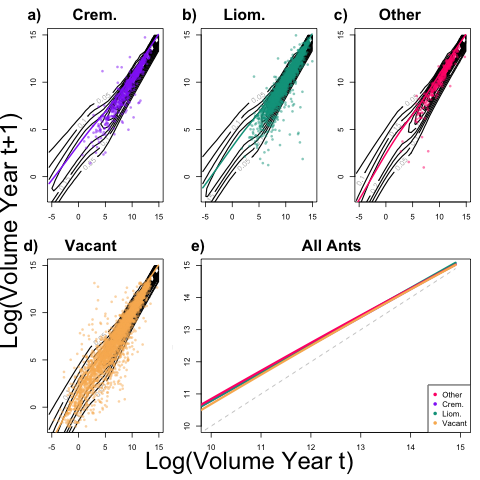
\includegraphics[width = 0.95\linewidth]{Figures/grow_contour.png}
	\caption{This figure shows the next predicted size of cholla based on previous size with each individual ant partner. The solid colored lines (seen in all panels) are the next mean predicted size of cholla. The points (seen in panels a-d) are the observed data which informs these estimates. The black countour lines (seen in a-d) appear at 5\% increments showing where 5\%, 10\%, etc. of the data is expected to fall. They grey dashed line (in panel e only) shows the line where the next predicted size is the same as the previous (aka there is no growth on this line and below this line is shrinkage). }
	\label{fig:Grow}
\end{figure}

\begin{figure}[H]
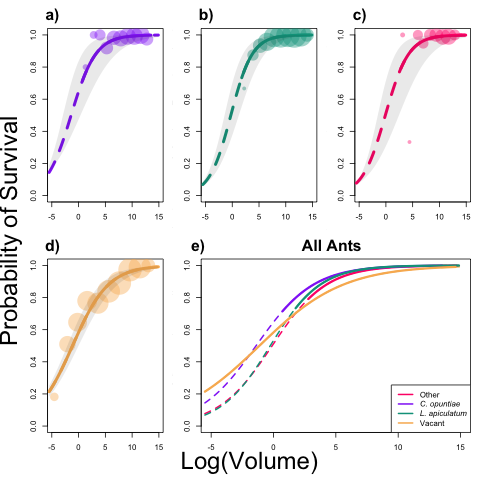
\includegraphics[width=0.95\linewidth]{Figures/survival_plot.png}
\caption{This figure shows the estimated survival rates based on the size of the cactus with each individual ant partner. The solid colored lines (shown on all panels) indicate the mean estimated survival rates. The dashed lines (shown in panel e) indicate extrapolations beyond existing data (where we estimated survival for plants tended by ants where we had never seen a tended cactus of that size). The grey area around the solid lines (shown in panels a-d) show the 90\% confidence interval for the estimates. The colored dots are the real data binned by size to show how our estimates align with real survival observations. A larger circle means we had more data on survival of plants of this size with this partner.}
\label{fig:Surv}
\end{figure}

We found evidence that ant visitation leads to increased floral viability rates and that ant identity can influence the strength of viability benefits.
We observed mean viability rates of flowers between 39\% and 96\% (Figure \ref{fig:viab}).
Ant partners influence the mean viability rate of flowers, with \textit{L. apiculatum}-tended plants experiencing the highest mean viability rate (86\%, Figure \ref{fig:Viab}b), followed by \textit{C. opuntiae} and Other tended plants (at 74-75\%, Figure \ref{fig:Viab}b,c), and vacant plants had the lowest floral viability rate (71\%, Figure \ref{fig:Viab}d).
Plants tended by \textit{L. apiculatum} had floral viability advantages, while plants in states of \textit{C. opuntiae}, Other ants, and vacancy had very similar floral viability rates. 


\begin{figure}[H]
	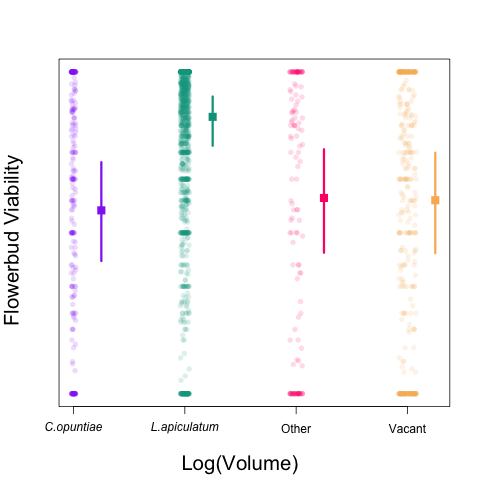
\includegraphics[width=0.95\linewidth]{Figures/viab.png}
	\caption{This figure shows the estimated distributions of floral viability rates compared to observed distributions of floral viability rates of cholla based on ant partner identity. The solid lines indicate the estimated viability distribution. The colored histograms represent the observed viability rates of plants with that partner. }
	\label{fig:Viab}
\end{figure}

We analyzed all other vital rates mentioned in the methods as well.
The results of each of these as well as the posterior predictive checks are all included in the Apendix A.

We analyzed the correlation coefficients of all models which included ant state as a predictor and found that the annually varying effects of each ant on survival were the least correlated, and that the effects on growth were the most correlated. 
Low correlation indicates synchronicity, which is necessary for portfolio effect to occur because a central thesis of this effect is that partners must react differently to temporal environmental stochasticity.
Across growth, survival, and viability models, the annally varying random effects of Other ants were the most asynchronous (the least correlated with the effects of other partners), while vacant random effects were the most synchronous. 
This variety of synchronicity across ant states and vital rates indicates there is potential for portfolio effect as many of the ants effects revealed low synchronicity, particularly in the survival model. 


\begin{figure}[H]
	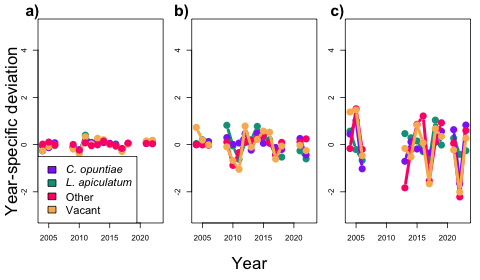
\includegraphics[width=0.95\linewidth]{Figures/year_ant_timeseries.png}
	\caption{This figure shows the mean affect of each ant partner on a) the estimated next size, b) the estimated survival, and c) the floral viability of cacti across every year of our study. These values are estimated from the fitted random effects of ant and year in our models. Each point represents the mean of the random effect of the identified model, ant, and year (e.g. the lowest dot in panel b) represents the mean effect of vacancy on survival rates in year 2011).}
	\label{fig:Annual_Ant}
\end{figure}
\ali{}{Honestly not sure if I should include an image for this one or just report some values? We should discuss. }

\subsection*{What are the frequency and direction of partner turnover across the plant life cycle?}
We found that 40\% of plants experienced an ant state transition on average, with very distinct size-dependence and directional patterns (Figure \ref{fig:Ant_Transition}). 
Vacancy is the most likely ant state of small plants ($\leq 10 log(cm^3)$).
Even when small plants are ant-tended at the start of the transition year, they are most likely to transition back to vacancy (Figure \ref{fig:Ant_Transition}b-d). 
The probability of becoming ant-tended increases with size, though it is not equally likely to be tended by all partners. 
For large plants that are initially vacant or tended by \textit{L. apiculatum} or Other ants, \textit{L. apiculatum} is the most likely next partner, suggesting that this partner species is able to colonize plants that were previously vacant or occupied by Other ants, and effectively retain plants that it previously occupied.  
\textit{C. opuntiae} were also able to retain plants they previously occupied, but not as well as \textit{L. apiculatum}: for plants that begin the transition year with \textit{C. opuntiae}, the probability that those plants remain occupied by \textit{C. opuntiae} at the end of the transition year is only slightly greater than the probability of take-over by \textit{L. apiculatum}, while take-over in the other directino is extremely rare. 
It is also notable that transitions away from the initial state of  \textit{L. apiculatum} were almost always transitions to vacancy (Figure \ref{fig:Ant_Transition}d), while transitions away from the initial states of \textit{C. opuntiae} and Other  were often transitions to other ants. 
This suggests a competitive hierarchy whereby \textit{L. apiculatum} may abandon low-value plants with litte nectar production but is almost never displaced from high-value plants. 

\begin{figure}[H]
	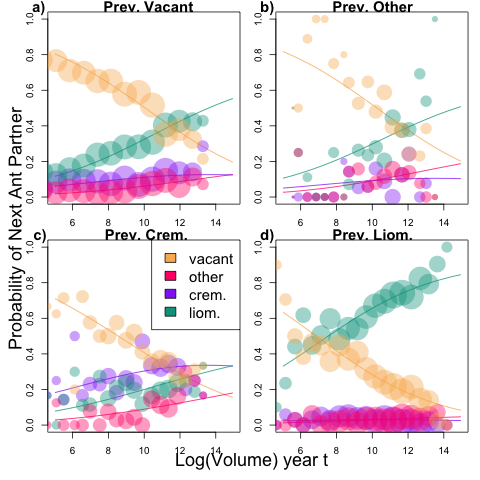
\includegraphics[width=0.95\linewidth]{Figures/transition.png}
	\caption{This figure shows the probability of being tended by each ant partner or vacant based on the size of the plant. Each panel shows these probabilities for a different previous ant state. The solid lines represent the mean probability of being tended by a specific partner. The colored points are the real data binned by size to show how our estimates align with real visitation observations. A larger circle means we had more data on visitation of plants of this size with this previous partner.}
	\label{fig:Ant_Transition}
\end{figure}

\subsection*{What is the net effect of partner diversity on plant fitness, and what mechanism(s) explain(s) this effect?}
By integrating vital rate results and ant transition dynamics into the multi-state IPM we can evaluate the fitness implications of different scenarios of partner diversity and identity. 
First, there was strong evidence that ant visitation had mutualistic fitness effects on plant partners. 
The lowest mean fitness was $\lambda_{S,Vacant}$, the fitness of the cholla with no partners (Figure \ref{fig:LambdaMeans}b).
Across all 1+ partner scenarios, we are *****(double check after final runs)82--100\% confident that any scenario of ant visitation elevates fitness. 
Furthermore, we find an apparent positive effect of partner diversity, with cactus fitness postive related to partner richness, averaging over partner identities (Figure \ref{fig:LambdaMeans}b).

\begin{figure}
	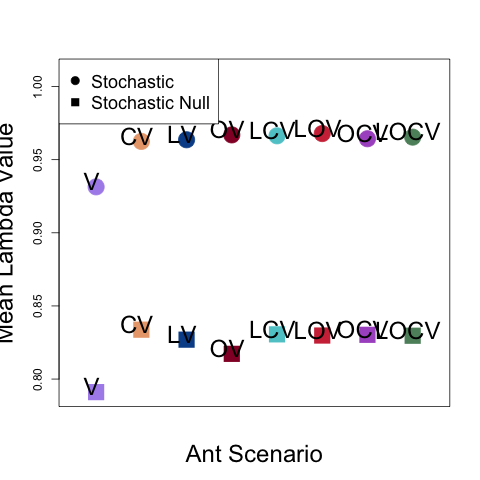
\includegraphics[width=0.61\linewidth]{Figures/comp_outputmeans_s_sn.png}
	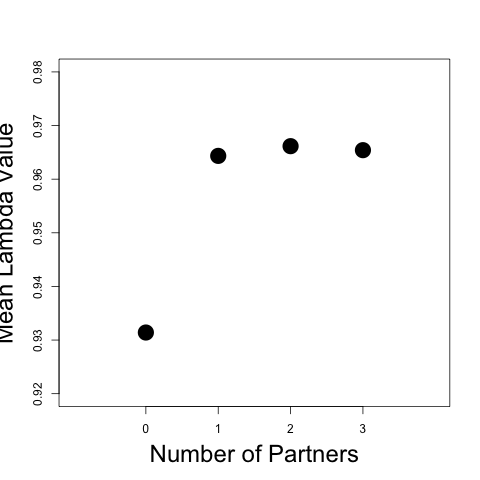
\includegraphics[width=0.39\linewidth]{Figures/comp_num_partners_s.png}
	\caption{Panel a) shows the mean values of the estimated $\lambda_{S}$ (filled in circles) and $\lambda_{SN}$ (empty circles with an X) for each simulated combination of ant partners. The letters above the points correspond to what ant partners are present (V = Vacant, C = \textit{C. opuntiae}, L = \textit{L. apiculatum}, O = other). Panel b) shows the mean values of the estimated $\lambda_{S}$ for }
	\label{fig:LambdaMeans}
\end{figure}

We originally believed the benefits of partner diversity are heavily driven by the presence of a single best partner rather than overall synergy.
However, we found that there was little benefit of any specific partner over another.
The identity and number of partners does not appear to significantly affect the fitness of the cacti. 
This indicates that while each of these partners are beneficial, there does not appear to be a significant benefit of partner diversity within this system. 

After further simulations, we found that this lack of diversity benefits are not driven by frequency of a single ant. 
Using the simulations where all ants had equal frequencies across sizes (further explained and analyzed in Appendix C), we found the same fitness patterns as in the competitive exclusion model described above.
Equal probability for transitioning into any ant state meant that the numbers of \textit{C. opuntiae} and Other ants were boosted significantly.
Despite this, the fitness of scenarios including these less frequent ants were not increased meaningfully.


We found no evidence of portfolio effect, meaning the presence of multiple partners did not buffer against the potentially negative effects of annual fluctuations.
The effect of all ant partners can be measured as $\lambda_{All} - \lambda_{Vacant}$ (Figure \ref{fig:Portfolio}).
We are are *****(double check after final runs)94\% confident that when all ants are present the cholla experience higher fitness than when no ants are present according to both the synchronized and non-synchronized model scnearios. 
When subtracting these two resulting vectors from each other (($\lambda_{S,All} - \lambda_{S,Vacant}$) - ($\lambda_{SN,All} - \lambda_{SN,Vacant}$)), we found that we are only *****(double check after final runs) 52\% confident that partners offer higher benefits when able to respond uniquely to a fluctuating environment. 
There is no real difference between the two scenarios, meaning we have no evidence of portfolio effect.

\begin{figure}
	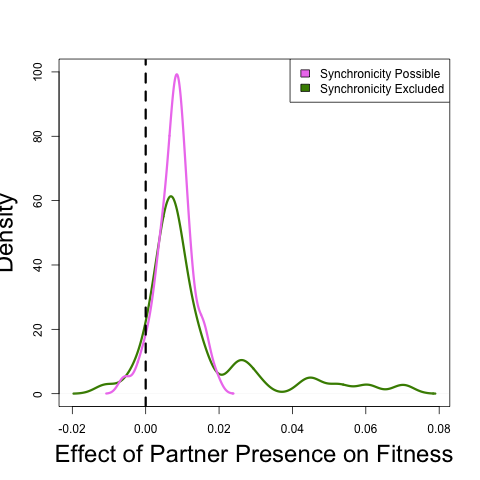
\includegraphics[width=\linewidth]{Figures/portfolio_effect.png}
	\caption{This figure shows the distribution of $\lambda_{S,All}-\lambda_{S,Vacant}$ in pink and $\lambda_{SN,All}-\lambda_{SN,Vacant}$ in green. The vertical dashed line shows where the effect of partners on the fitness of the cholla is 0 (to the left the partners have a negative effect, to the right the partners are beneficial).}
	\label{fig:Portfolio}
\end{figure}



\section*{Discussion}\ali{}{I am struggling reframing this part. I think I may need to start with a new outline, because a lot of what we had doesn't apply to our new conclusions that mutualism is good but we don't see a benefit of partner diversity?}
% mini abstract paragraph
Mutualisms commonly involve multiple partners but the ecological consequences of partner diversity remain poorly understood. 
Here we show that partner identity can play an important role in determining both vital rates and population fitness. 
The results of our heirarchical models revealed that different ant partners had different effects on vital rates, with \textit{C. opuniae} tended plants experiencing advantages in growth and survival when small, and \textit{L. apiculatum} tended plants experiencing floral viability advantages.
The results of our stochastic IPM revealed that all diversity scenarios which included partners resulted in the highest possible fitness for tree cholla, suggesting that partner diversity may not be beneficial or negative in this system. 
The results of our stochastic null IPM revealed that there is no evidence of portfolio effect in our system. 
These results highlight that partner presence can increase the overall benefits of a focal mutualism without synergistic benefits and the importance of a mechanistic understanding to explain the benefits of diversity across systems. \ali{}{This may not be great, but I am struggling a bit with this framing}

% Connect to broader patterns in the lit
Similar studies have reported complementarity \citep{Palmer2010,Rezende2007,Hooper2005,Cardinale2007,Afkhami2021} while we found that neither complementarity nor sampling effect explains the benefits of diversity in our system. 
In our first round of results, focused on individual ant effects on vital rates, we found that different ant partners affected different vital rates uniquely (Figures \ref{fig:Grow},\ref{fig:Surv},\ref{fig:Viab}).
This indicated to us that we may be dealing with complementarity, and that each ant partner offered a unique form of herbivore protection across ontogeny and or across different processes. 
However, our IPM results showed that we were actually observing a lack of beneficial diversity, leaving us with questions about how these results could fit together. 


%This may have to do with the sheer number of \textit{L. apiculatum} in the system.
%None of these cited studies reported a single species with overwhelming frequency within their systems.
%In most cases of complementarity, there are relatively similar frequencies of each partner, which is not the case in our system. 
%75\% of observed ants are \textit{L. apiculatum} in our system, while only 17\% are \textit{C. opuntiae}.
%Our vital rate results suggested we may find evidence of complementarity, with \textit{C. opuntiae} appearing to boost growth and survial and \textit{L. apiculatum} appearing to boost floral viability.
%We believe there may simply not be enough \textit{C. opuntiae} in the system to have complementarity, leading instead to sampling effect driven by the overwhelming frequency of one ant.


% If there is one best partner then diversity should impose opportunity costs
%In systems where there is a single "best" partner and concurrent partner interactions, theory suggests that diversity should lead to more interactions with the best partner, thereby increasing the fitness of the focal mutualist \citep{Batstone2018}.
%In systems with mutually exclusive partner interactions and a "best`` partner,  theory suggests that diversity should impose an opportunity cost of the form of interacting with "inferior" partners, meaning scenarios where more than just the best partner is available should result in decreased fitness \citep{Noe1994}.
%While out system is aligned with this second expectation, we did not see any decreased fitness from the single "best" partner scenario to scenarios with the "best" partner and other ants included. 
%We do not see this reflected in our IPM results, potentially because of the high frequency of \textit{L. apiculatum}, the "best" partner, across the population.
%In the mutually exclusive interaction scenario, the fitness of the population should essentially be an average of the fitness conferred by each partner weighted by their frequency. 
%Due to the much higher frequency of \textit{L. apiculatum} ants, we believe the weighted average is almost equivalent to that of the single ant scenario with \textit{L. apiculatum} present. 


%Turnover
Partner turnover is likely a significant driver behind the fitness we see within cholla populations, however the processes which drive the actual turnover frequency and directions remain a mystery in this system.
In the literature, it is clear that the frequency of partner turnover can have big effects on the fitness of the focal mutualist \cite{Fiala1994, Horvitz1986, Oliveira1999, Sachs2004}.
In some systems high freqency of turnover is necessary for resiliency and leads to higher fitness benefits \cite{Trojelsgaard2015}, while in other systems loyalty is the most beneficial \cite{Batstone2018}.
We found that some ants had higher frequency of turnover than others, specifically the other category appeared to have high frequency of turnover, rarely returning to the same plant, while \textit{C. opuntiae} and \textit{L. apiculatum} often returned.
The direction of partner turnover is also important when the identity of partners impacts the quality of benefits recieved \cite{Fonseca2003, Alonso1998, Dejean2008, Noe1994}.
In our study we found that there are distinct patterns to the direction of partner turnover. 
Specifically, most plants are tended by \textit{L. apiculatum} ants at some point, because vacant plants, other tended plants, and \textit{L. apiculatum} tended plants are all most likely to be tended by \textit{L. apiculatum} ants.
This indicates that while \textit{L. apiculatum} ants are loyal to their own plants and return multiple years in a row to the same ones, they are also strong colonizers. 

What now remains is to determine the underlying processes that lead to the emergence of these characterized patterns. 
Throughout the literature, it is reported that non-symbiotic ants and non-mutualist ants are highly attracted to monosaccharide heavy EFN \citep{Heil2004,Kautz2009} and that plants often produce monosaccharide EFN to avoid exploitation \citep{Heil2010}.
It has been previously reported that when reproducing, the nectar of stem segments has a greater disaccharide vs monosaccharide ratio, while flowerbuds have a lower ratio \citep{Miller2008}. 
This could potentially have a significant impact on the partners who tend a plant in a given season, though determining the impacts of nectar on directional turnover requires further study. 
We conducted alternative simulations where the driving mechanism for ant occupation was not competitive exclusion, these results are included in Apendix XX.

% Portfolio Effect
Our work explcitly incorporated temporal environmental stochasticity, which raises the opportunity for portfoilio effect as a mechanism of diversity benefits. Yet, we find no evidence of portfolio effect within our system. 
When partners exhibit different reactions to varying environments, interacting with multiple partners can lead to more consistent benefits across time \citep{Batstone2018}.
In our system, we do not directly measure the reactions of ant partners to temporal environmental stochasticity, rather we measure the effects of each partner on the cholla across time, allowing us to statistically quantify how the benefits recieved from each partner vary across time.
We found that each ant partner had different effects on different vital rates across time,  indicating they exhibit different reactions to varying environments, leading us to believe that portfolio effect could be possible in this system. 
We compared the fitness of cholla under simulations where the variation in benefits across time reflected what we found in nature to siulations where each ant was forced to react the same way to temporal variation (excluding the possibility of portfolio effect).
We found the benefits were not stronger across time when the ants were allowed to vary naturally than when they were forced to react synchronously, indicating that portfolio effect does not explain the benefits of diversity in our system.
Other portfolio effect studies \citep{Lazaro2022,Tornos2023} found 
One study \cite{Dallas2021} found that while portfolio effect was easy to show in theoretical models, it is often very weak or nonexistent in empirical data across many systems. 
This indicates that it may be very difficult to detect, disguised by different mechanisms, or uncommon in real systems.

% Value of Long-term data
This paper shows the importance of long-term datasets in investigating species interactions and calls for further use of long-term data. 
Previously studies have analyzed how partner identity and partner turnover impact focal mutualist fitness \cite{Fonseca2003, Dejean2008, Noe1994, Barrett2015, Bruna2014, Trojelsgaard2015}.
Separate studies have analyzed how inter-annual variability impacts focal mutualists \cite{Alonso1998, Alarcon2008, Ollerton2006, Horvitz1990, Lazaro2022}.
The long term dataset we used gave us the unique ability to consider the combined effects of partner identity, partner turnover, and temporal stochasticity.

First, we were able to look at many years of data to reveal the complex dynamics of partner turnover and identity, revealing that the frequency of \textit{L. apiculatum} may be primarily responsible for the fitness of the cholla rather than any other ant partner observed.
Fewer years of data would not have been able to show the distinct patterns of \textit{L. apiculatum} taking over cacti that were previously tended by any other partners with as much clarity.
Second, our long-term data set allowed us to test the portfolio effect.
This data is required, because we must show that the partners react asynchronously to temporal environmental stochasticity for portfolio effect to even be possible.
This is a great example of how long-term data may offer more power to test underlying mechanisms in similar systems.
Finallly, previous studies by \cite{Miller2007} hypothesized that \textit{C. opuntiae} may be a parasite based on the effects on the cholla cacti.
Using more years of consecutive data in this system, we were able to show that \textit{C. opuntiae}, while the worst individual partner in terms of the overall cholla fitness (Figure \ref{fig:LambdaMeans}), increases the growth and survival rates of cacti prior to reproduction.
The length of our data set has allowed us to dive into individual vital rates as well as overall fitness with more clarity.


% Herbivory
Herbivory is an important driver of the fitness of cholla in this system, as herbivores directly impact the growth, survival, and reproductive efforts of the cacti.
Despite this, we do not directly account for herbivory in our system. 
Rather, we assume that herbivory can be captured in the effects they have on growth, survival, and reproductive effort observations.
In the future, further studies on the direct impacts of herbivory would bolster the results reported here and expand our knowledge within this system.
This is particularly true in light of our consideration of portfolio effect. 
In the same way that different species of ants likely react to temporal environmental variation differently, the same can be said for herbivores \citep{Thibaut2012}.
Herbivores have variations in their population reflective of the environment changing temporally, meaning there are "good" and "bad" years for herbivores just like for ant defenders \citep{Batstone2018}, so the strength of their negative effect varies. 
The fluctuations in herbivore populations in conjunction with ant-specific defenses agains herbivores provide a solid foundation to study portfolio effect in this system. 
We found no evidence of this mechanism (Figure \ref{fig:Portfolio}), but a more herbivore explicit model in the future may reveal more about driving mechanisms. 


% Limitations
As with any study, there are limitations to consider when interpreting the results reported here.
These results are based on observational data regarding ant effects on plant demography rather than experimental data, meaning we are able to determine correlations but not causation.
We are able to report evidence that plants experience higher growth when associating with a particular partner, but we are not able to determine if the presence of the ant is the cause of the higher growth observed.
It is possible, for example, that plants which attract \textit{L. apiculatum} through osition have a different pattern of resource allocation to growth and survival and this is what we are observing rather than a direct affect of \textit{L. apiculatum} on the plant.
This is a typical limitation of observational studies, but does not reduce the power or importance of our results, just the interpretation.
However, we believe that the ants likely have direct impacts on the plant demography based on other studies which find the presence of ants can lead to direct increases in survival \citep{Beattie1985}, reproductive efforts \citep{Ford2015}, growth \citep{Frederickson2005}, etc.
In the future, it would be interesting to verify the causation of our results through experimental manipulations.
One further expansion could include nectar analysis of these cacti in conjuntion with ant interactions to look not only at the ant parnter impacts on the plant demography, but also at the ability of plants to attract specific partners through nectar composition shifts. 

Another limitation of our study is that we are simulating populations through an IPM to estimate fitness, meaning we have to extrapolate beyond observed interaction.
In our study, small plants are rarely seen with partners, yet we report on the expected effects of each ant on the growth and survival of plants from the size of new recruits to the largest plants. 
While we are confident in our model, there remains the small possibility of interactions which have never been observed occurring (such as a seedling tended by \textit{L. apiculatum}).
This means that our fitness estimations are based on extrapolations of our observed data, and while we have done what we can to be confident in our model, it is possible that our assumptions that observed patterns would continue beyond observed interactions could be incorrect.
Another example of this includes our single partner simulations.
We have no data on what the fitness of cholla would look like if the only ant partner possible was \textit{C. opuntiae}, yet we offer an estimation based on the effects of this partner in a diverse system.
The many years of data and 10467 unique plant-year observations included in our analysis allow us to have relatively high confidence in our outputs despite extrapolations.




\section*{Acknowledgments}
This should be drafted.
%%%%%%%%%%%%%%%%%%%%%
% Statement of Authorship
%%%%%%%%%%%%%%%%%%%%%
% This section should also be commented out while your MS is undergoing
% double-blind review. The specifics should of course be adapted to
% your paper, but the paragraph below gives some hints of possible
% contributions.

\section*{Data and Code Availability}
This should be drafted.


\renewcommand{\theequation}{A\arabic{equation}}
% redefine the command that creates the equation number.
\renewcommand{\thetable}{A\arabic{table}}
\setcounter{equation}{0}  % reset counter 
\setcounter{figure}{0}
\setcounter{table}{0}

%%%%%%%%%%%%%%%%%%%%%
% Bibliography
%%%%%%%%%%%%%%%%%%%%%
% You can either type your references following the examples below, or
% compile your BiBTeX database and paste the contents of your .bbl file
% here. The amnatnat.bst style file should work for this---but please
% let us know if you run into any hitches with it!
%
% If you upload a .bib file with your submission, please upload the .bbl
% file as well; this will be required for typesetting.
%
% The list below includes sample journal articles, book chapters, and
% Dryad references.
\bibliographystyle{apalike}
\bibliography{References.bib}


\newpage{}

\section*{Tables}
\renewcommand{\thetable}{\arabic{table}}
\setcounter{table}{0}

\renewcommand{\thetable}{\arabic{table}}
\setcounter{table}{0}

% I am creating a table here to include all parameter estimations and descriptions
  \begin{table}[]
  \begin{tabular}{l|l|l}
    \textbf{Parameter} & \textbf{Median ($95\%$ CI)} & \textbf{Prior Distribution} \\
    \hline
    %% Growth Parameters
    growth xi intercept vacant $\beta_{01}^g$ & $-5.210899 (-5.686865, -5.491787)$ & sDE\\
    growth xi intercept other $\beta_{02}^g$ & $-5.8288 (-5.956217, 1.766021) $&asdf \\
    growth xi intercept \textit{C. opuntiae} $\beta_{03}^g$ & $-4.529523 (-6.0770390, 0.1222112)$ & asdf\\
    growth xi intercept \textit{L. apiculatum} $\beta_{04}^g$ & $-5.106802 (-5.4499944, 0.5453901)$ & asdf\\
    growth xi size dependent vacant $\beta_{11}^g$ & asdf&asdf \\
    growth xi size dependent other $\beta_{12}^g$ & asdf&asdf \\
    growth xi size dependent \textit{C. opuntiae} $\beta_{13}^g$ & asdf&asdf \\
    growth xi size dependent \textit{L. apiculatum} $\beta_{14}^g$ &sadf &asdf \\
    growth omega intercept $\omega_0^g$ & & \\
    growth omega size dependent $\omega_1^g$ & & \\
    growth alpha intercept $\alpha_0^g$ & & \\
    growth alpha size dependent $\alpha_1^g$ & & \\
    \hline
    %% Germination Parameters
    1-year germination intercept $\alpha^{\gamma_1}$ & & \\
    2-year germination intercept $\alpha^{\gamma_2}$ & & \\
    \hline
    %% Survival Parameters
    survival intercept vacant $\beta_{01}^s$ & & \\
    survival intercept other $\beta_{02}^s$ & & \\
    survival intercept \textit{C.opuntiae} $\beta_{03}^s$ & & \\
    survival intercept \textit{L. apiculatum} $\beta_{04}^s$ & & \\
    survival size dependent vacant $\beta_{11}^s$ & & \\
    survival size dependent other $\beta_{12}^s$ & & \\
    survival size dependent \textit{C. opuntiae} $\beta_{13}^s$ & & \\
    survival size dependent \textit{L. apiculatum} $\beta_{14}^s$ & & \\
    \hline
    %% Probability of Flowering Parameters
    flowering intercept $\beta_0^f$ & & \\
    flowering size dependent $\beta_1^f$ & & \\
    \hline
    %% Floral Viability Parameters
    viability intercept vacant $\beta_01^v$ & & \\
    viability intercept other $\beta02^v$ & & \\
    viability intercept \textit{C. opuntiae} $\beta_03^v$ & & \\
    viability intercept \textit{L. apiculatum} $\beta_04^v$ & & 

  \end{tabular}
  \caption{This table includes the median estimates, the 95$\%$ confidence intervals, and the prior distribution for each parameter in each model.}
  \label{tab:Params}
  \end{table}

\section*{Figure legends}



\section*{Appendix A: Additional Methods and Parameters}
In addition to the models described in the body of the paper, we fit several other simpler models using data from previous studies.
These models are described below.

\paragraph{Seeds Per Fruit}
With data\cite{Miller2006}, we fit a model for the number of seeds produced by every fruit on a cholla ($\kappa(a')$) in year $t+1$ based on the ant partner $a'$ in year $t+1$.
We fit this model to seed data $y^{\kappa}$ using a Negative Binomial distribution and the log link function: 
$$y^{\kappa} \sim  Negative Binomial(\hat{\kappa},\hat{\phi})$$
%$$ \hat{\kappa } = \beta_{0}^{\kappa} \times a'$$
$$\hat{\phi} = \beta_{0}^{\phi}$$
The data used for this model did not include data on ants in the ``other" category, so we used the data from vacant plants to parameterize seeds per flower for plants with ``other" ants in the IPM.

\paragraph{Recruit Size Distribution}
%The recruit size model ($n(x',a')$) estimates the size distribution of all recruits } from a given year $t+1$, with no fixed or random effects. 
We fit this model to recruit size data $y^{\eta}$ using a Normal distribution with the identity link function: 
$$y^{\eta} ~\sim N(\hat{\eta},\hat{\sigma})$$
%$$\hat{\eta} = \beta_{0}^{\eta}$$
where $\hat{\sigma}$ is estimated with a non-informative prior. 

\paragraph{Germination}
With germination data \cite{Miller2007}, we fit two models for the probability of germinating from the first year seedbank ($\gamma_1$) or the second year seedbank ($\gamma_2$) in year $t+1$, with no fixed or random effects.
These models were fit to germination data $y^{\gamma_1}, y^{\gamma_2}$  using the binomial distribution with logit link functions:
$$y^{\gamma_1} \sim Binomial(\hat{\gamma_1})$$
$$y^{\gamma_2} \sim Binomial(\hat{\gamma_2})$$
%$$logit(\hat{\gamma_1}) = \beta_{0}^{\gamma_1}$$
%$$logit(\hat{\gamma_2}) = \beta_{0}^{\gamma_2}$$

\paragraph{Pre-Census Survival}
With recruit census data \cite{Miller2006}, we fit a model for the probability of a seedling (which germinates in early Fall) surviving to when we census in May ($\delta$) of year $t+1$ (accounting for missed mortality events), with fixed effects of the previous size $x$ and random effects of the transect $m$.
We fit this model to pre-census survival data $y^{\delta}$ using a Bernoulli distribution with a logit link function: 
$$y^{\delta} ~ Bern(\hat{\delta})$$
%$$logit(\hat{\delta}) = \beta_{0}^{\delta} + m$$
where $m \sim N(0, \sigma_{transect}^2)$ is the random effect of transect where the recruited individual was analyzed for survival.


\section*{Appendix B: Observed Herbivory Data}
One type of data we took every year is herbivory data, which involved looking at the plant for evidence of recent herbivory (fresh bites) and noting the type and quantity of herbivores observed.


\section*{Appendix C: Alternative Ant Transition Simulations}
In addition to the competitive exclusion model defined and analyzed in the body of the paper, we simulated results from several other potential models. 
We chose to include competitive eclusion as our primary results in the paper because we believe it to be the most biologically realistic.
However, in building and testing of alternative models we found that the method of ants occupying plants significantly impacts the fitness of the population. 
We tested two alternative transition models, one called the frequency based model and one called the equal likelihood model. 

\paragraph{Frequency Based Model}
The first alternative hypothesis we tested was what we called the frequncy based model.
In this model rather than the proportion of vacant cacti being maintained, the proportion of cacti occupied by each species is maintained and when one is removed it is replaced with vacancy.
This version of the model assumes that the frequency of each ant we see is reflective of the real frequency of populations rather than some other mechanism.
With this model we found very clear evidence of Sampling Effect in the system. 
When only  \textit{C. opuntiae}, Other ants, or both ants are present, there is very little difference in the fitness of the cacti from when no partners are present. 
Only when \textit{L. apiculatum} ants are present do we see an increase in the fitness of the focal mutualist (Figure \ref{fig:FreqLambdaMeans}a).
In this simulation, the more partners that are present the higher the fitness of the focal mutualist is, confirming that partner diversity would be beneficial through sampling effect if this transition model were correct.  (Figure \ref{fig:FreqLambdaMeans}b).

\begin{figure}
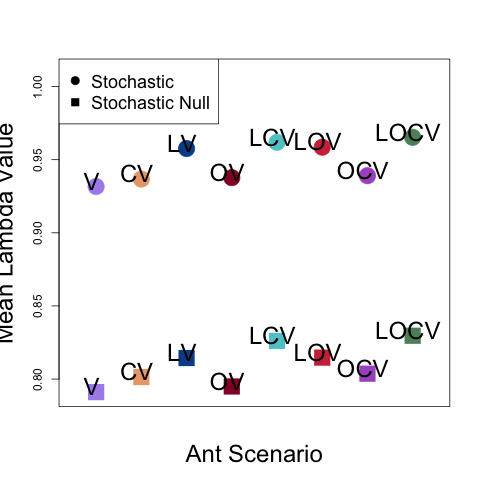
\includegraphics[width=0.61\linewidth]{Figures/freq_outputmeans_s_sn.png}
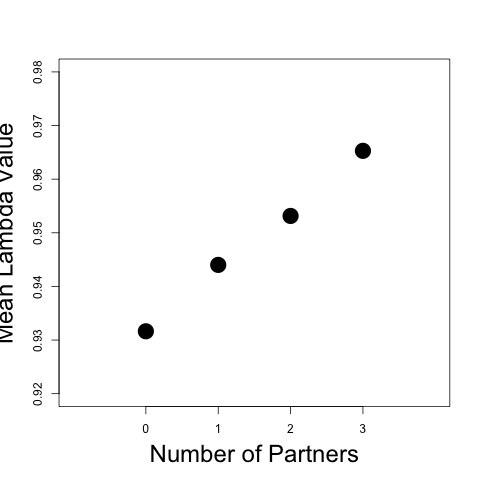
\includegraphics[width=0.39\linewidth]{Figures/freq_num_partners_s.png}
\caption{Panel a) shows the mean values of the estimated $\lambda_{S}$ (filled in circles) for each simulated combination of ant partners. The letters above the points correspond to what ant partners are present (V = Vacant, C = \textit{C. opuntiae}, L = \textit{L. apiculatum}, O = other). Panel b) shows the mean values of the estimated $\lambda_{S}$ for }
\label{fig:FreqLambdaMeans}
\end{figure}

\paragraph{Equal Likelihood Model}
The second alternative hypothesis we tested was what we called the equal likelihood model.
In this model we preserved the observed pattern of size-dependent vacancy/occupancy, but occupancy was manipulated to be equally likely for all partner identities. 
This was designed to remove the effect overwhelming numbers of \textit{L. apiculatum} ants may have. 
Despite very different proportions, we found very similar outcomes to the competitive exclusion model analyzed in the paper. 
All ants are beneficial, but having more than one is not necessarily any better than having an individual species as a partner (Figure \ref{fig:BetweenLambdaMeans}a).
Partner presence is beneficial, but neither identity nor number of partners appears to be important (Figure \ref{fig:BetweenLambdaMeans}b).

\begin{figure}
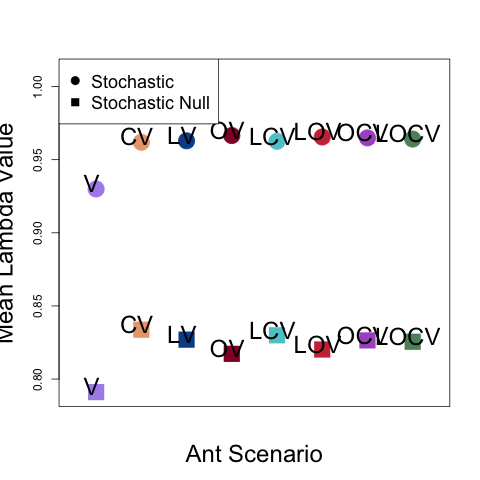
\includegraphics[width=0.61\linewidth]{Figures/equal_outputmeans_s_sn.png}
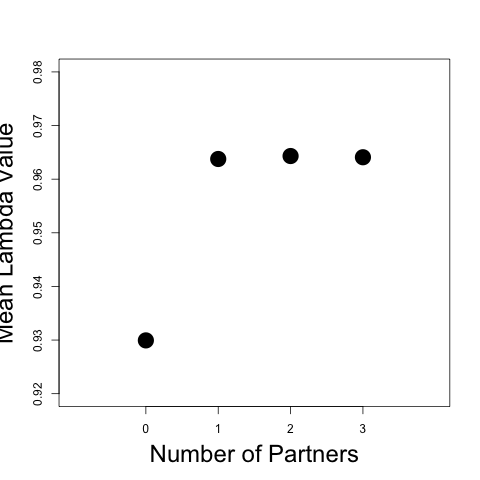
\includegraphics[width=0.39\linewidth]{Figures/equal_num_partners_s.png}
\caption{Panel a) shows the mean values of the estimated $\lambda_{S}$ (filled in circles) for each simulated combination of ant partners. The letters above the points correspond to what ant partners are present (V = Vacant, C = \textit{C. opuntiae}, L = \textit{L. apiculatum}, O = other). Panel b) shows the mean values of the estimated $\lambda_{S}$ for }
\label{fig:BetweenLambdaMeans}
\end{figure}


\section*{Appendix D: Posterior Checks and Model Validation}
For each model fitted, we conducted two tests to determing if the fit was acceptable to use in our IPM. 
First, we checked the convergence of each parameter.
Below we show the convergence of all $\beta$ terms listed in the Statistical Modeling subsection of Methods.
Second, we checked the posterior fit, comparing the estimated values of each model to the $y$ values of the actual data.
We show these posterior checks below, split by ant partner where relevant.
%% Growth Figure
%% Survival Figure
\begin{figure}
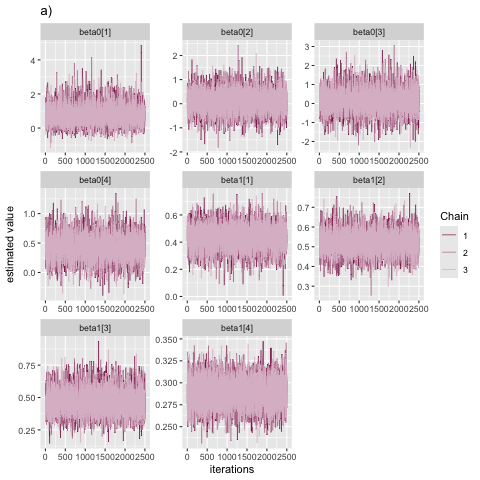
\includegraphics[width = 0.45\linewidth]{Figures/surv_conv.png}
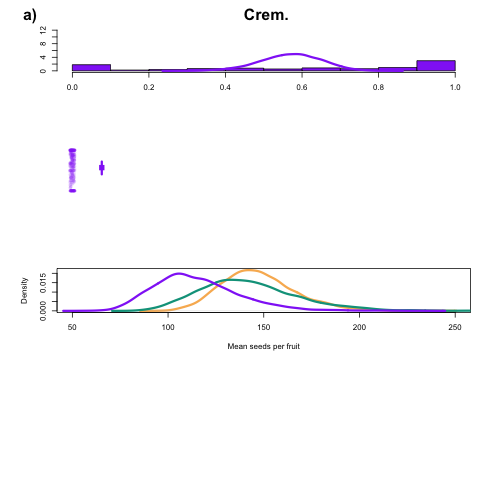
\includegraphics[width=0.45\linewidth]{Figures/surv_post.png}
\caption{The a) posterior convergence of the parameters estimated by the survival model and the b) posterior distribution of survival estimates (pink lines) for each ant species (1 = \textit{C. opuntiae}, 2 = \textit{L. apiculatum}, 3 = other, 4 = vacant) compared to the mean survival distribution (black line) of the real data.}
\label{fig:Surv_post}
\end{figure}
%% Reproduction Figure
\begin{figure}
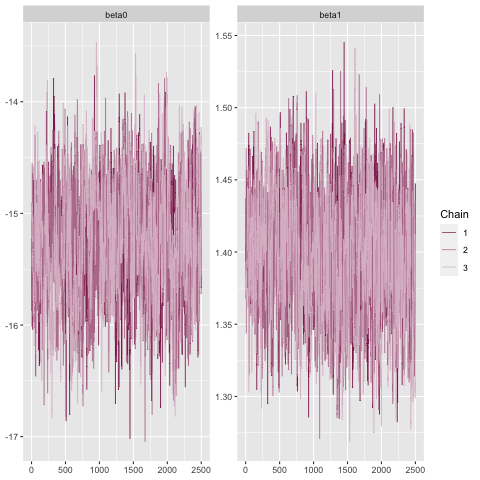
\includegraphics[width = 0.45\linewidth]{Figures/repro_conv.png}
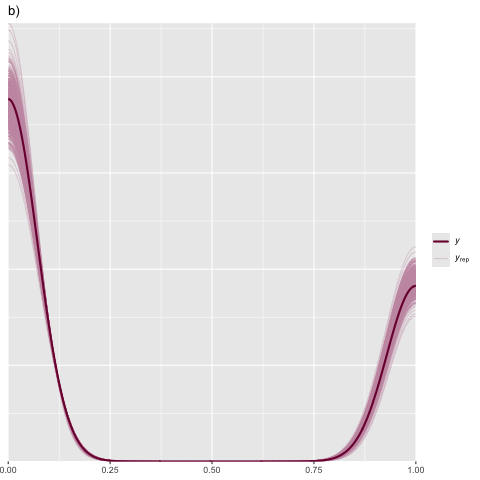
\includegraphics[width=0.45\linewidth]{Figures/repro_post.png}
\caption{The a) posterior convergence of the parameters estimated by the reproduction model and the b) posterior distribution of reproductive status estimates (pink lines) for each ant species (1 = \textit{C. opuntiae}, 2 = \textit{L. apiculatum}, 3 = other, 4 = vacant) compared to the mean reproductive status distribution (black line) of the real data.}
\label{fig:Repro_post}
\end{figure}
%% Flowering Figure
\begin{figure}
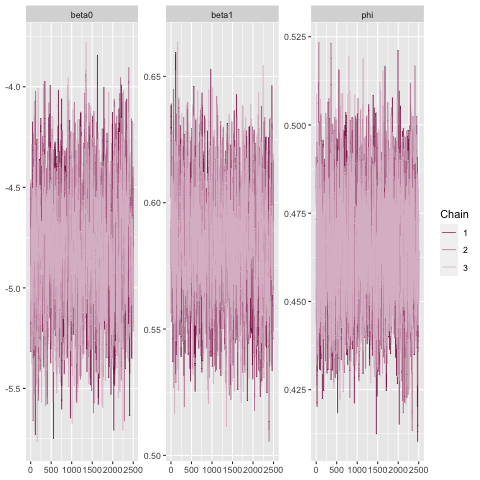
\includegraphics[width = 0.45\linewidth]{Figures/flow_conv.png}
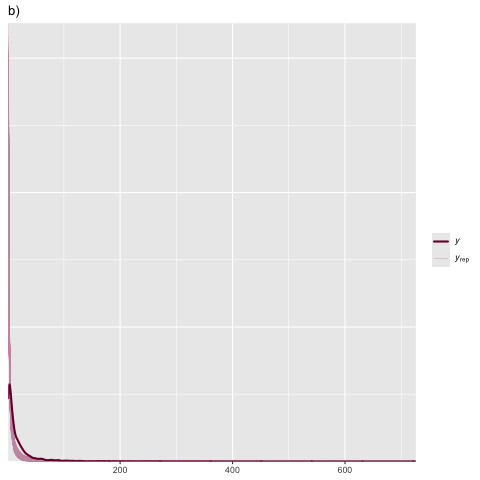
\includegraphics[width=0.45\linewidth]{Figures/flow_post.png}
\caption{The a) posterior convergence of the parameters estimated by the number of flowers model and the b) posterior distribution of the number of flowers estimated (pink lines) compared to the mean distribution of observed flowers (black line).}
\label{fig:Flow_post}
\end{figure}
%% Viability Figure
\begin{figure}
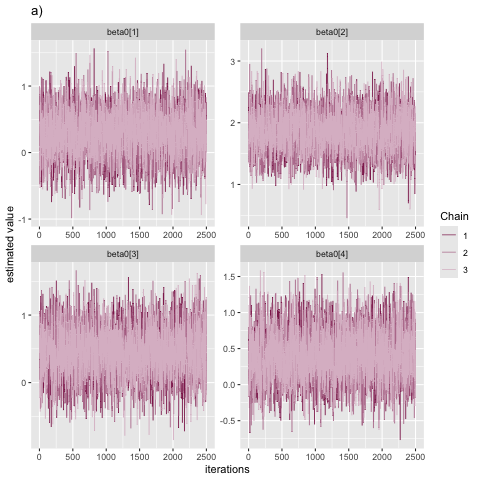
\includegraphics[width = 0.45\linewidth]{Figures/viab_conv.png}
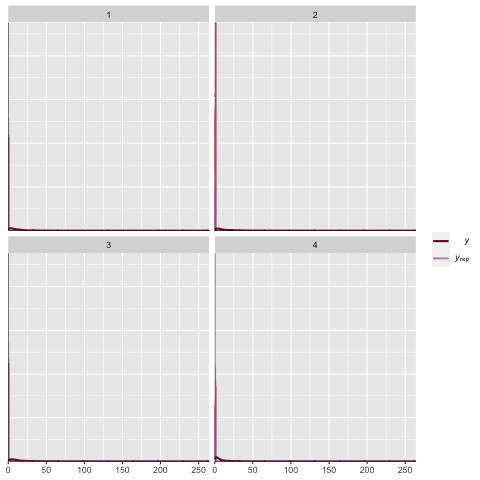
\includegraphics[width=0.45\linewidth]{Figures/viab_post.png}
\caption{The a) posterior convergence of the parameters estimated by the viability model and the b) posterior distributions of floral viability estimates (pink lines) for each ant species (1 = \textit{C. opuntiae}, 2 = \textit{L. apiculatum}, 3 = other, 4 = vacant) compared to the mean floral viability distribution (black line) of the real data.}
\label{fig:Viab_post}
\end{figure}
%% Seeds Per Fruit
\begin{figure}
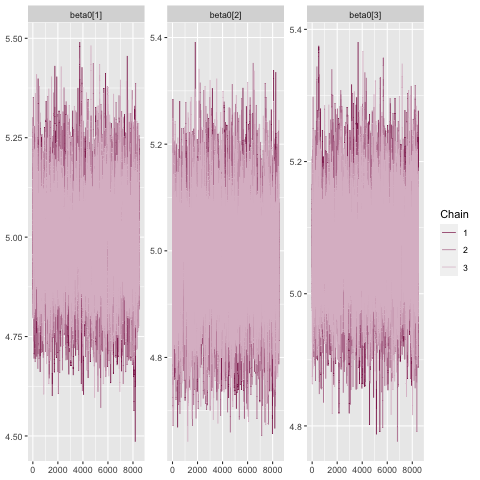
\includegraphics[width = 0.45\linewidth]{Figures/seed_conv.png}
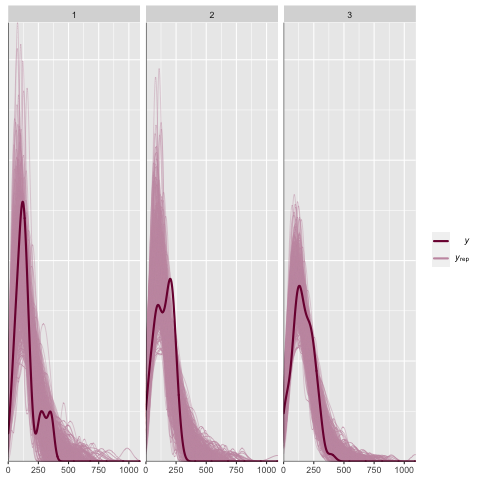
\includegraphics[width=0.45\linewidth]{Figures/seed_ant_post.png}
\caption{The a) posterior convergence of the parameters estimated by the seeds per fruit model and the b) posterior distributions of seeds per fruit estimates (pink lines) for each ant species (1 = \textit{C. opuntiae}, 2 = \textit{L. apiculatum}, 3 = vacant) compared to the mean seeds per fruit distribution (black line) of the real data.}
\label{fig:seed_post}
\end{figure}
%% Fruit survival 
% \begin{figure}
%% 	\includegraphics[width = 0.45\linewidth]{Figures/                .png}
%% 	\includegraphics[width=0.45\linewidth]{Figures/               .png}
% 	\caption{The a) posterior convergence of the parameters estimated by the fruit survival model and the b) posterior distributions of fruit survival estimates (pink lines) compared to the mean fruit survival distribution (black line) of the real data.}
% 	\label{fig:fruit_surv_post}
% \end{figure}
% %% Ant Transitions
% \begin{figure}
%% 	\includegraphics[width = 0.45\linewidth]{Figures/             .png}
%% 	\includegraphics[width=0.45\linewidth]{Figures/               .png}
% 	\caption{The a) posterior convergence of the parameters estimated by the ant transitions model and the b) posterior distributions of next ant partners estimates (pink lines) for each previous ant species (1 = \textit{C. opuntiae}, 2 = \textit{L. apiculatum}, 3 = other, 4 = vacant) compared to the mean next ant partner distribution (black line) of the real data.}
% 	\label{fig:Transitions_post}
% %% Germination
\begin{figure}
	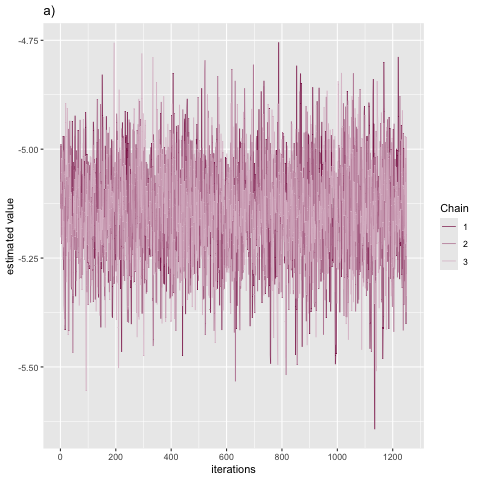
\includegraphics[width = 0.45\linewidth]{Figures/germ1_conv.png}
	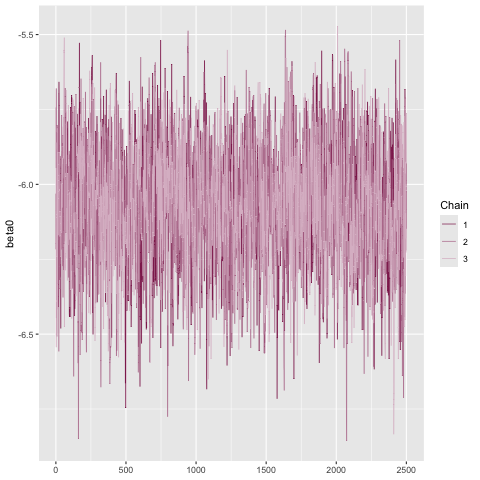
\includegraphics[width=0.45\linewidth]{Figures/germ2_conv.png}\\
	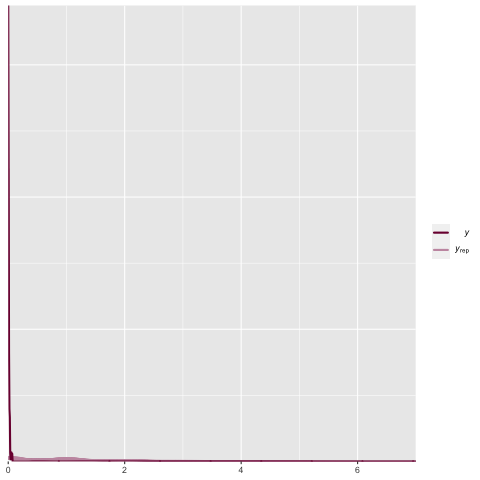
\includegraphics[width=0.45\linewidth]{Figures/germ1_post.png} 	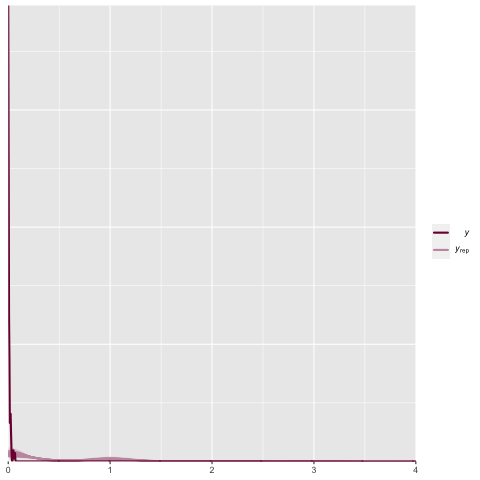
\includegraphics[width=0.45\linewidth]{Figures/germ2_post.png}
	\caption{The a-b) posterior convergence of the parameters estimated by the germination from year one seedbank and germination from year two seedbank models respectively. The c-d) posterior distributions of floral viability estimates (pink lines) compared to the mean germination distribution (black line) of the real data for first year germinants and second year germinants respectively.}
	\label{fig:Germ_post}
\end{figure}

%% Pre-Census Survival
\begin{figure}
	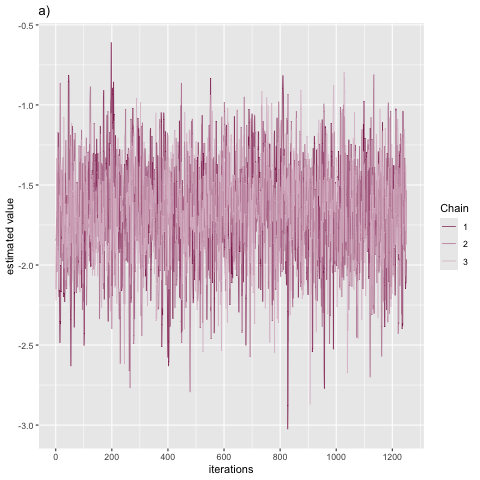
\includegraphics[width = 0.45\linewidth]{Figures/seed_surv_conv.png}
	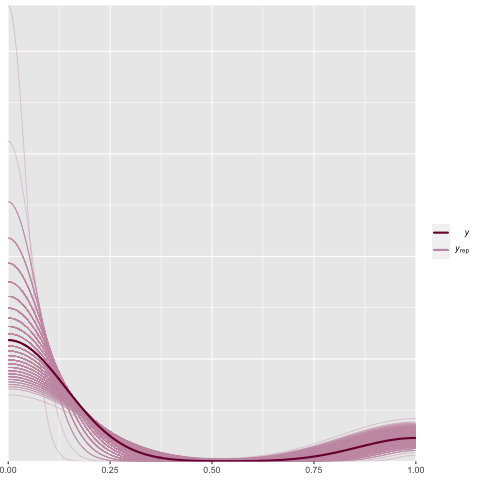
\includegraphics[width=0.45\linewidth]{Figures/seed_surv_post.png}
	\caption{The a) posterior convergence of the parameters estimated by the pre-census survival model and the b) posterior distribution of the pre-census survival estimated (pink lines) compared to the mean distribution of observed pre-census survival (black line).}
	\label{fig:Pre_Surv_post}
\end{figure}
%%

\subsection*{Statistical Models -- Results}
Below are the results reorted of all statistical models not described in the main body of the text. 

%% Reproduction Model
\paragraph{Reproduction Model}
The probability of a plant reproducing in a given year is highly size dependent. 
The mean probability of reproducing remains at about 0\% until the plant reaches a medium size, after which the mean probability of reproducing increases steadily before reaching about 100\% at large sizes. 



%% Seeds Produced
\paragraph{Seeds Per Flower Model}
Each viable flower on a plant produces between 97 and 257 seeds.
\tom{This number is affected by the ant partner present. 
	\textit{C. opuntiae} tended plants produce a mean of 148 seeds per flower. 
	\textit{L. apiculatum} tended plants produce a mean of 149 seeds per flower. }{These results are not consistent with Ohm and Miller, where Crem had lower seeds than Liom. I would check this. This section should also reference that paper because these are not new results.}
Vacant plants produce a mean of 160 seeds per flower. 
We are 73\% and 78\% confident that vacant plants produce more seeds per flower on average than plants tended by \textit{C. opuntiae} and \textit{L. apiculatum} ants respectively.


\tom{%% Precensus Survival\
	\paragraph{Precensus Survival Model}
	Pre-census seed survival rates fall between 0\% and 95\% with the mean pre-census seed survival at 18\%.
	
	%% Germination
	\paragraph{Germination Model}
	Seeds have a significantly higher probability of germinating in year one than in year two.
	Seeds in year one experience germination rates between 50\% and 100\% with a mean of 62\% germination.
	Seeds in year two experience germination rates between 50\% and 98\% with a mean of 58\% germination.
	
	
	%% Recruit size distribution
	New recruits are expected to be between the sizes of 0.11 $cm^3$ and 0.38 $cm^3$ with a mean size of 0.20 $cm^3$.}{Move to an appendix. These results are not relevant for the questions at hand.}




\end{document}
